% $Header: /cvsroot/latex-beamer/latex-beamer/solutions/generic-talks/generic-ornate-15min-45min.en.tex,v 1.5 2007/01/28 20:48:23 tantau Exp $

\documentclass{beamer}
%\documentclass[mathsherif]{beamer}

% This file is a solution template for:

% - Giving a talk on some subject.
% - The talk is between 15min and 45min long.
% - Style is ornate.



% Copyright 2004 by Till Tantau <tantau@users.sourceforge.net>.
%
% In principle, this file can be redistributed and/or modified under
% the terms of the GNU Public License, version 2.
%
% However, this file is supposed to be a template to be modified
% for your own needs. For this reason, if you use this file as a
% template and not specifically distribute it as part of a another
% package/program, I grant the extra permission to freely copy and
% modify this file as you see fit and even to delete this copyright
% notice.


\mode<presentation>
{
\usecolortheme[RGB={89,165,140}]{structure}

  \usetheme{Warsaw}
\setbeamercolor*{palette quaternary}{fg=white,bg=structure!40!black}


% o Singapore
% \setbeamercolor{normal text}{bg=blue!10} % para azul, la oscuridad del color se regula cambiando (!20)
% \beamertemplateshadingbackground{yellow!50}{magenta!50} % degradado de amarillo a magenta
  % or ...
% \setbeamertemplate{navigation symbols}{} quitar l\'{\i}nea de s\'{\i}mbolos esquina inferior derecha -in\'{u}tiles
  \setbeamercovered{transparent}
  % or whatever (possibly just delete it)
}


\usepackage[spanish]{babel}
% or whatever

\usepackage[utf8]{inputenc}
% or whatever

\usepackage{times}
\usepackage[T1]{fontenc}
\usepackage{lmodern}

%\usepackage{lucidaso}
%\usepackage[small]{eulervm}

% Paquetes de David
\usepackage{verbatim}
\usepackage{listings}
\usepackage{color}
\usepackage{etoolbox}
\usepackage{xstring}
\usepackage{../gsi-parametros}
 
\definecolor{dkgreen}{rgb}{0,0.6,0}
\definecolor{gray}{rgb}{0.5,0.5,0.5}
\definecolor{mauve}{rgb}{0.58,0,0.82}
  
\lstset{ %
  language=C,                % the language of the code
  basicstyle=\footnotesize,           % the size of the fonts that are used for the code
  %numbers=left,                   % where to put the line-numbers
  numberstyle=\tiny\color{gray},  % the style that is used for the line-numbers
  numbersep=5pt,                  % how far the line-numbers are from the code
%  backgroundcolor=\color{white},      % choose the background color. You must add \usepackage{color}
  showspaces=false,               % show spaces adding particular underscores
  showstringspaces=false,         % underline spaces within strings
  showtabs=false,                 % show tabs within strings adding particular underscores
  %frame=single,                   % adds a frame around the code
  rulecolor=\color{black},        % if not set, the frame-color may be changed on line-breaks within not-black text (e.g. commens (green here))
  tabsize=2,                      % sets default tabsize to 2 spaces
  captionpos=b,                   % sets the caption-position to bottom
  breaklines=true,                % sets automatic line breaking
  breakatwhitespace=false,        % sets if automatic breaks should only happen at whitespace
  %title=\lstname,                   % show the filename of files included with \lstinputlisting;
  keywordstyle=\color{blue},          % keyword style
  commentstyle=\color{dkgreen},       % comment style
  stringstyle=\color{mauve},         % string literal style
  escapeinside={\%*}{*)},            % if you want to add a comment within your code
  morekeywords={*,...}               % if you want to add more keywords to the set
}


% Or whatever. Note that the encoding and the font should match. If T1
% does not look nice, try deleting the line with the fontenc.

% para Singapore
%\setbeamertemplate{footline}{%
%\leavevmode%
%\hbox{%
%\begin{beamercolorbox}[wd=.333333\paperwidth,ht=2.25ex,dp=1ex,center]{author in head/foot}%
%\usebeamerfont{author in head/foot}\insertshortauthor
%\end{beamercolorbox}%
%\begin{beamercolorbox}[wd=.333333\paperwidth,ht=2.25ex,dp=1ex,center]{title in head/foot}%
%\usebeamerfont{title in head/foot}\insertshorttitle
%\end{beamercolorbox}%
%\begin{beamercolorbox}[wd=.333333\paperwidth,ht=2.25ex,dp=1ex,right]{date in head/foot}%
%\usebeamerfont{date in head/foot}\insertshortdate{}\hspace*{2em}
%\insertframenumber{} / \inserttotalframenumber\hspace*{2ex}
%\end{beamercolorbox}}%
%\vskip0pt%
%}
%
% para Warsaw
\newcommand*\oldmacro{}%
\let\oldmacro\insertshorttitle%
\renewcommand*\insertshorttitle{%
  \oldmacro\hfill%
  \insertframenumber\,/\,\inserttotalframenumber}

%\renewcommand*{\appendixname}{Referencias}


\title[Investigación y políticas de publicación] % (optional, use only with long paper titles)
{Investigación y políticas de publicación}

%\subtitle
%{} % (optional)

\author[\asignatura] % (optional, use only with lots of authors)dvanced Robot Control
{\autor}
% - Use the \inst{?} command only if the authors have different
%   affiliation.

\institute[Universidad de Alcal\'{a}] % (optional, but mostly needed)
{
  %\inst{1}%
  \textcolor{structure} {\emph{\textbf{Departamento de Autom\'{a}tica}}}\\
  Universidad de Alcal\'{a}

% - Use the \inst command only if there are several affiliations.
% - Keep it simple, no one is interested in your street address.

%\date[Short Occasion] % (optional)
%{Date / Occasion}

\vspace*{0.5cm}

\includegraphics[height=0.8cm]{comun/uah}
}
\date{}



%logos s\'{o}lo en title
\titlegraphic{
  
\includegraphics[scale=0.45]{comun/dpto}
  \hfill
 % 
\includegraphics[scale=0.35]{gso1}
 % \hfill
  
\includegraphics[scale=0.20]{comun/gso1}
}

% logos tal cual: salen en todos los frames...
%\pgfdeclareimage[height=0.4cm]{left-logo}{gso1}
%\pgfdeclareimage[height=0.4cm]{right-logo}{gso1}
%\logo{\pgfuseimage{right-logo}}


%\setbeamertemplate{sidebar left}
%{
%\logo{\pgfuseimage{left-logo}}
%\vfill%
%\rlap{\hskip0.1cm\insertlogo}%
%\vskip15pt%
%}

\subject{Talks}
% This is only inserted into the PDF information catalog. Can be left
% out.



% If you have a file called "university-logo-filename.xxx", where xxx
% is a graphic format that can be processed by latex or pdflatex,
% resp., then you can add a logo as follows:


% marca de agua de una imagen

\usebackgroundtemplate{
\includegraphics[width=\paperwidth]{comun/marcadeagua}}


%% QUITAR LOS PARES %% DE LAS L\'{I}NEAS DE \AtBeginSubsection PARA QUE SE GENERE LA NAVEGACI\'{O}N EN LA SUBSECCIONES
%%\AtBeginSubsection[]
%% {
%%     \begin{frame}{\'{I}ndice}
%  \small
%  \tableofcontents[currentsection,hideothersubsections]
%  \normalsize
% \end{frame}

%%    \small
%%    \tableofcontents[currentsection,currentsubsection]
     % \tableofcontents[pausesections]
%%   \end{frame}
%%}

%% QUITAR LOS PARES %% DE LAS L\'{I}NEAS DE \AtBeginSubsection PARA QUE SE GENERE LA NAVEGACI\'{O}N EN LA SUBSECCIONES
%%\AtBeginSection[]
%% {
%%     \begin{frame}{\'{I}ndice}
%  \small
%  \tableofcontents[currentsection,hideothersubsections]
%  \normalsize
% \end{frame}

%%    \small
%%    \tableofcontents[currentsection]
     % \tableofcontents[pausesections]
%%   \end{frame}
%%}

% If you wish to uncover everything in a step-wise fashion, uncomment
% the following command:

%\beamerdefaultoverlayspecification{<+->}


\begin{document}

\begin{frame}[plain]
  \titlepage
\end{frame}

\begin{frame}[shrink]{Table of Contents}
 \frametitle{Table of Contents}
 \tableofcontents

 % no me vale: deja descolgado el cap\'{\i}tulo 4
 % \frame[allowframebreaks]%
 %    {\frametitle{\'{I}ndice}\tableofcontents[part=4]}
  % You might wish to add the option [pausesections]
\end{frame}


% Since this a solution template for a generic talk, very little can
% be said about how it should be structured. However, the talk length
% of between 15min and 45min and the theme suggest that you stick to
% the following rules:

% - Exactly two or three sections (other than the summary).
% - At *most* three subsections per section.
% - Talk about 30s to 2min per frame. So there should be between about
%   15 and 30 frames, all told.

\section{Introducción}
\subsection{¿Qué es investigar?}

\begin{frame}[plain]
	\begin{center}
	\begin{columns}
	\column{.6\textwidth}
	\begin{block}{}
	\begin{center}
	¿Qué es investigar?
	\end{center}
	\end{block}
	\end{columns}
	\end{center}
\end{frame}

\begin{frame}{Introducción}{¿Qué es investigar?}
	\begin{columns}
		\column{.6\textwidth}
 		   \begin{itemize}
			\item Ideas relacionadas
	   			\begin{itemize}
				\item Conocimiento, metodología, experimentación, observación, teoría, ...
			    \end{itemize}
			\end{itemize}
		\column{.4\textwidth}
  			\begin{center}
      		
\includegraphics[width=1\textwidth]{figs/ciencia.png}
	    	\end{center}
		\end{columns}
	
    	\begin{itemize}
		\item \alert{Investigar es crear conocimiento}
  			\begin{itemize}
			\item No es \textit{aprender}: Aprender es pasivo, la investigación es activa
			\item No es \textit{innovar}: Innovar es crear un nuevo producto o servicio
   			\end{itemize}
    	\end{itemize}
\end{frame}

\subsection[Motivación]{Motivación}

\begin{frame}[plain]
	\begin{center}
	\begin{columns}
	\column{.6\textwidth}
	\begin{block}{}
	\begin{center}
	¿Por qué investigar?
	\end{center}
	\end{block}
	\end{columns}
	\end{center}
\end{frame}

\begin{frame}{Introducción}{¿Por qué investigar?}
	\centering Funciones de la univ.: \alert{Captar}, \alert{transmitir} y \alert{generar} conocimiento

	\begin{columns}
	\column{.5\textwidth}
	\begin{block}{Motivos académicos}
	\begin{center}
		Mejora la docencia\\
		\alert{Excelencia académica}\\
		Autoaprendizaje\\
		Prestigio
	\end{center}
	\end{block}
	\column{.5\textwidth}
	\begin{block}{Motivos económicos}
		\begin{center}
		Soluciona problemas\\
		Base de la innovación\\
		\alert{Fuente de ingresos}\\
		\textit{Spin-off}\\
		\end{center}
	\end{block}
	\end{columns}

	\vspace{0.25cm}
	\centering \alert{La investigación mejora la sociedad}

	\begin{itemize}
		\item Fases de la investigación
			\begin{enumerate}
			\item Plantear una pregunta
			\item Plantear una respuesta
			\end{enumerate}
		\item ¿Vale cualquier pregunta y cualquier respuesta?
	\end{itemize}
\end{frame}

\subsection[Método científico]{Método científico}

\begin{frame}{Introducción}{Método científico}
  	 \vspace{-0.2cm}
	 La ciencia es, ante todo, un \alert{método}
		\begin{itemize}
			\item No es un conjunto de verdades incuestionables	
		\end{itemize}
  	 \vspace{-0.3cm}
 	 \begin{center}
   		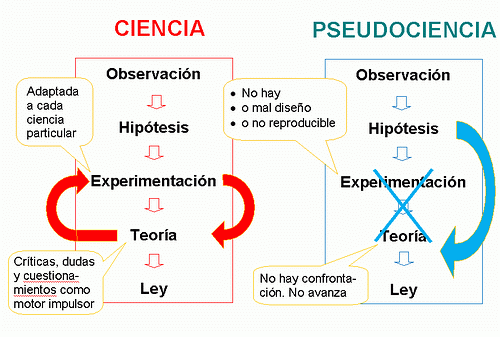
\includegraphics[width=0.7\textwidth]{figs/metodo.png}
   	 \end{center}
\end{frame}

\subsection[Comunicación]{La comunicación científica}

\begin{frame}{Introducción}{La comunicación científica}
	\vspace{-0.3cm}
	\begin{center}
	\begin{columns}
	\column{.6\textwidth}
	\begin{block}{}
	\begin{center}
	``Si he visto más lejos ha sido porque he subido a hombros de gigantes''\\
    \texttt{Isaac Newton}
	\end{center}
	\end{block}
	\end{columns}
	\end{center}
    \begin{itemize}
	\item ¿Qué sucede cuando se descubre algo?
	    \begin{itemize}
			\item Hay que compartirlo: \alert{PUBLICAR}
			\item No existe investigación sin publicación
			\item Es una medida de calidad
				\begin{itemize}
					\item En innovación hay patentes
					\item En programación hay líneas de código
					\item En ciencia hay publicaciones
				\end{itemize}
			\item Publicar requiere de habilidades específicas difíciles de obtener
				\begin{itemize}
					\item Es un objetivo fundamental de un doctorado
				\end{itemize}
	    \end{itemize}
    \end{itemize}
\end{frame}

\section{Introducción a la publicación}

\subsection{Tipos de publicaciones}

\begin{frame}{Introducción a la publicación} {Tipos de publicaciones}
	\begin{columns}
		\column{.5\textwidth}
		Tipos: Congreso, revista, \textit{workshop}, libro y capítulo de libro
			\begin{itemize}
			\item Sólo consideramos los dos primeros
			\end{itemize}
		Elementos comunes:
		\begin{itemize}
			\item \alert{Revisión entre pares}
			\item Necesidad de \alert{ISBN}
		\end{itemize}

		\column{.5\textwidth}
	 	\begin{center}
	  	  
\includegraphics[width=\linewidth]{figs/peerReview.jpg}
 	 	\end{center}
	 \end{columns}
\end{frame}

\subsection{Congreso}

\begin{frame}{Introducción a la publicación} {Tipos de publicaciones: Congreso}
	\begin{columns}
		\column{.5\textwidth}
			\begin{block}{Tipos de contribuciones}
				\begin{center}
					Póster\\
					Short paper\\
					Full paper
				\end{center}
			\end{block}

		\column{.5\textwidth}
			\begin{block}{Tipos de congreso}
				\begin{center}
				Nacional\\
			 	Internacional\\
				\textit{Workshop} (nac./int.)
				\end{center}
			\end{block}
		\end{columns}

		\begin{itemize}
			\item Trabajo sin finalizar
			\begin{itemize}
				\item Resultados preliminares
				\item Trabajo urgente
			\end{itemize}
			\item Extensión corta (8 págs.)
			\item Publicación rápida (meses)
			\item Revisión informal (según congreso)
			\item Se publican actas
			\item \textit{Call for papers}
			\item Web imprescindible: \url{http://www.wikicfp.com/cfp/}
 		\end{itemize}
\end{frame}

\subsection{Revista}

\begin{frame}{Introducción a la publicación} {Tipos de publicaciones: Revista (I)}
	\begin{columns}
		\column{.5\textwidth}
			\begin{block}{Tipos de artículo}
				\begin{center}
				Full paper\\
				Otros: Review, position, revisión de libro, agenda, ...
				\end{center}
			\end{block}
		\column{.5\textwidth}
			\begin{block}{Números especiales}
				Temáticas muy específicas, a veces asociado a un congreso
			\end{block}
	\end{columns}
	\vspace{0.5cm}
	\begin{itemize}
		\item Trabajos cerrados: Resultados definitivos y detallados
		\item Extensión larga, según revista
		\item Publicación lenta (1 año) y revisión formal (según revista)
		\item \textit{Normalmente, ampliación de un artículo de congreso}
	\end{itemize}
\end{frame}

\begin{frame}{Introducción a la publicación} {Tipos de publicaciones: Revista (II)}
	\begin{columns}
		\column{.7\textwidth}
			\begin{block}{Coste de la subscripción}
				\scriptsize{
				\begin{table}[h]
				\begin{center}
				\begin{tabular}{ll}
				\hline\noalign{\smallskip}
				 		& Coste \\
				\noalign{\smallskip} 
				\hline 
				\noalign{\smallskip}
				ACS inorganic journals 			& 8.974  \\ 
				RCS inorganic journals 			& 7.520	 \\ 
				Wiley-VCH inorganic journals	& 17.991 \\ 
				Elsevier inorganic journals		& 33.884 \\ 
				\noalign{\smallskip} 
				\hline
				\noalign{\smallskip} 
				TOTAL							& 68.369 \\ 
				\noalign{\smallskip} 
				\hline
				\end{tabular}
				\end{center}
				\end{table}
			}

		\end{block}
	\end{columns}
	\vspace{0.5cm}
\end{frame}

\begin{frame}[plain]{Introducción a la publicación} {Tipos de publicaciones: Revista (III)}
	\vspace{-0.1cm}
 	 \begin{center}
   		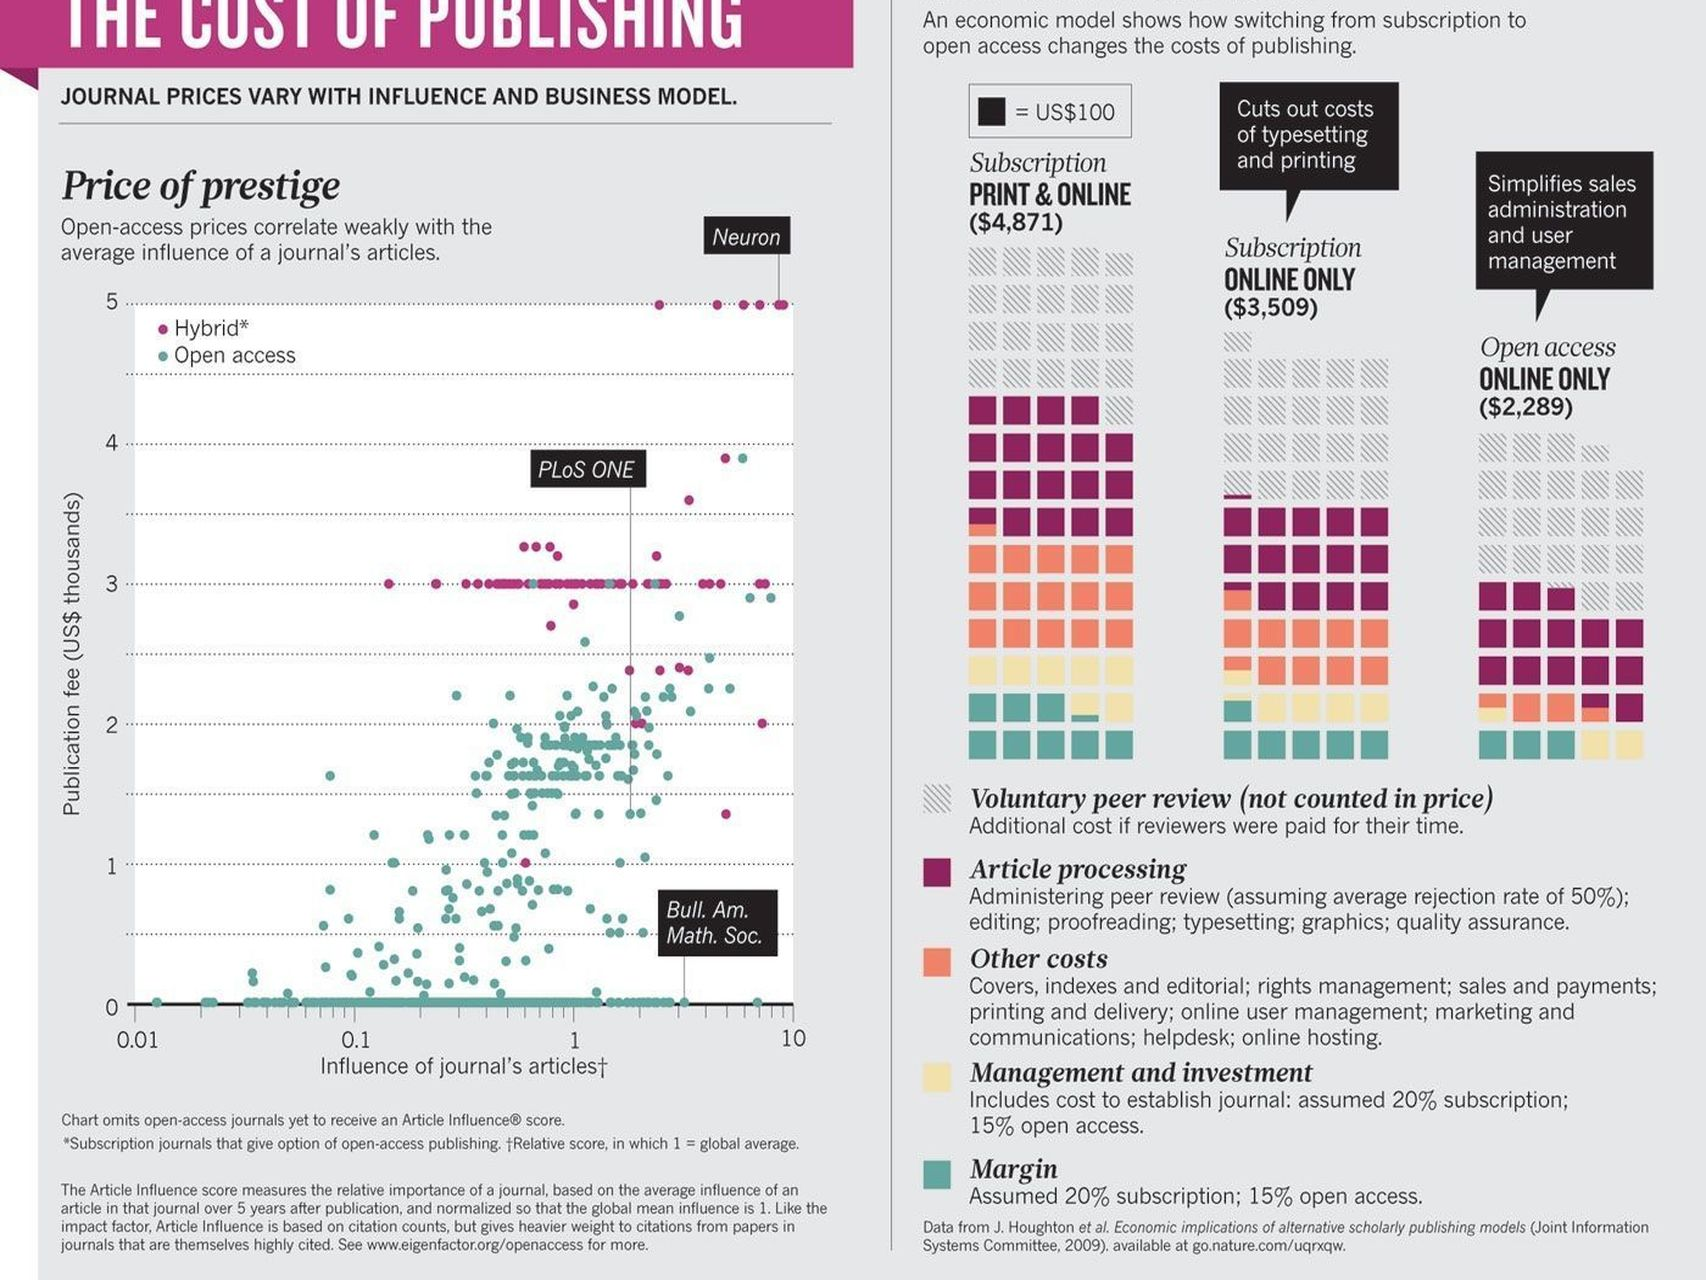
\includegraphics[width=0.9\textwidth]{figs/openaccess.jpg}\\\tiny{(Source: Nature)}\\
	 \normalsize{¿Cómo identificar las buenas publicaciones?}
	\end{center}
\end{frame}


\section[Métricas]{Métricas de calidad}
\subsection{Revista}

\begin{frame}{Métricas de calidad}{Revistas (I)}
  	\begin{itemize}
		\item Medir la calidad de una publicación es fundamental
			\begin{itemize}
			\item Publicar en buenas revistas es extremadamente difícil
			\end{itemize}
		\item Objetivo: Maximizar la repercusión del trabajo
			\begin{itemize}
			\item ¿Cómo saber el prestigio de una revista?: Número de citas
			\end{itemize}
		\item Concepto fundamental: \alert{Índice de impacto}
			\begin{itemize}
			\item Número de citas medio de una revista en los dos últimos años
			\end{itemize}
	\end{itemize}

	\begin{columns}
	\column{.6\textwidth}
 
	\begin{center}
	\vspace{-0.7cm}
	\begin{block}{Ejemplo: IEEE TEC 2011}
		\scriptsize{
		\begin{table}[h]
		\begin{center}
		\begin{tabular}{lll}
		\hline 
		 		& Citas & Artículos \\ 
		\hline
		2010	& 79 	& 54		\\ 
		2009	& 352 	& 75		\\ 
		\hline
		TOTAL	& 431	& 129		\\ 
		\hline
		\end{tabular}
		\end{center}
		\end{table}
	}
		\smallskip
		\centering $\text{IMPACTO: }\frac{431}{129}=3.341$
		\end{block}
	\end{center}
	\end{columns}
\end{frame}

\begin{frame}{Métricas de calidad}{Revistas (II)}
	\begin{columns}
	\column{.6\textwidth}
 	\begin{itemize}
		\item Significado del impacto
			\begin{itemize}
			\item Prestigio de una revista
			\item Cómo de buena es una revista
			\item Publicar con el máximo impacto
			\end{itemize}
		\item ¿Quién calcula el impacto?
			\begin{itemize}
			\item En una palabra: Empresas
			\item Las revistas \textit{no} intervienen
			\end{itemize}
		\item JCR (\textit{Journal Citation Report})
			\begin{itemize}
			\item Creado por \textit{Thomson-Reuters}
			\item Es la referencia absoluta
			\item Acceso de pago (muy caro)
			\end{itemize}
	\end{itemize}

	\column{.4\textwidth}
	\begin{center}
		\begin{block}{Referencia}
			\scriptsize{
			\begin{table}[h]
			\begin{center}
			\begin{tabular}{ll}
			%\hline 
			% 		& JCR \\ 
			%\hline
			Mínimo tesis doctoral	& 1	\\ 
			Buena tesis doctoral	& 2	\\ 
			Excelente tesis doctoral& 3	\\ 
			Contratado doctor		& 5	\\ 
			Titular de Universidad	& 8	\\ 
			Catedrático				& 20\\ 
			\end{tabular}
			\end{center}
			\end{table}
		}
		\end{block}
	\end{center}
	\end{columns}
\end{frame}

\begin{frame}{Métricas de calidad}{Revistas (III)}
	\begin{center}
	\begin{columns}
	\column{\textwidth}
	\begin{block}{Categorías en Computer Science del JCR}
		COMPUTER SCIENCE, ARTIFICIAL INTELLIGENCE\\
		COMPUTER SCIENCE, CYBERNETICS\\
		COMPUTER SCIENCE, HARDWARE \& ARCHITECTURE\\
		COMPUTER SCIENCE, INFORMATION SYSTEMS\\
		COMPUTER SCIENCE, INTERDISCIPLINARY APPLICATIONS\\
		COMPUTER SCIENCE, SOFTWARE ENGINEERING\\
		COMPUTER SCIENCE, THEORY \& METHODS
	\end{block}
	\end{columns}
	\end{center}
\end{frame}

\begin{frame}{Métricas de calidad}{Revistas (IV)}
	 \begin{center}
	    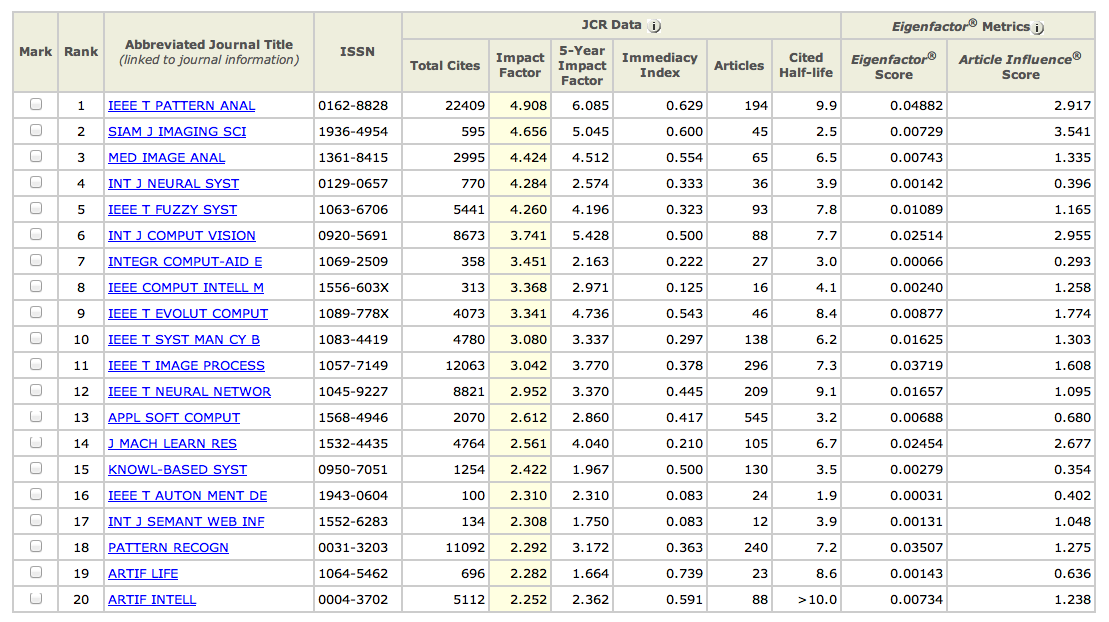
\includegraphics[width=1\linewidth]{figs/jcr.png}
 	 \end{center}
\end{frame}

\begin{frame}{Métricas de calidad}{Revistas (V)}
	Otras métricas
  	\begin{itemize}
		\item Cuartiles (Q1, Q2, Q3, Q4)
		\item Terciles (T1, T2, T3)
		\item Índice inmediato
		\item Índice a cinco años
		\item Posición en el JCR
	\end{itemize}
	Alternativa abierta al JCR: Scimago (\url{http://www.scimagojr.com/})
  	\begin{itemize}
		\item Acceso libre
		\item Resultados muy aprecidos al JCR
	\end{itemize}
\end{frame}

\subsection{Congreso}

\begin{frame}{Métricas de calidad}{Congreso}
  	\begin{itemize}
		\item Menos formal que el JCR
		\item CORE (\textit{Computing Research \& Education})
			\begin{itemize}
			\item Tres categorías: A, B y C
			\item Una categoría especial: A+
			\item Acceso libre en \url{http://core.edu.au/index.php/categories/conference\%20rankings/1}
			\end{itemize}
	\end{itemize}
\end{frame}

\subsection{Personal}

\begin{frame}{Métricas de calidad}{Personales (I)}
  	\begin{itemize}
		\item Número de citas
			\begin{itemize}
			\item Un artículo \textit{normal} tiene alguna decena de citas (o ninguna)
			\item Un \textit{buen} artículo puede tener cientos de citas
			\item Un artículo \textit{excepcional} del orden de varios miles (o una decena)
			\end{itemize}
		\item Índice H (o índice \textit{Hirsch})
			\begin{itemize}
			\item Mide productividad e impacto
			\item Utiliza los artículos más citados
			\item Un H5 significa que se tienen cinco artículo citados cinco veces
			\item La tendencia es usar H
			\end{itemize}
	\end{itemize}
\end{frame}

\begin{frame}{Métricas de calidad}{Personales (II)}
	\begin{center}
	\begin{columns}
	\column{\textwidth}
	\begin{block}{Referencia}
		H20, 20 años: Científico con éxito\\
		H40, 20 años: Científico excepcional (universidad de élite)\\
		H60, 20 años: Científicos únicos (Einstein tiene H93)
	\end{block}
	\alert{En general, un investigador ``normal'' tiene un H igual a los años que tenga de doctor}
	\end{columns}
	\end{center}
\end{frame}

\begin{frame}[plain]{Métricas de calidad}{Personales (III)}
	\begin{center}
      	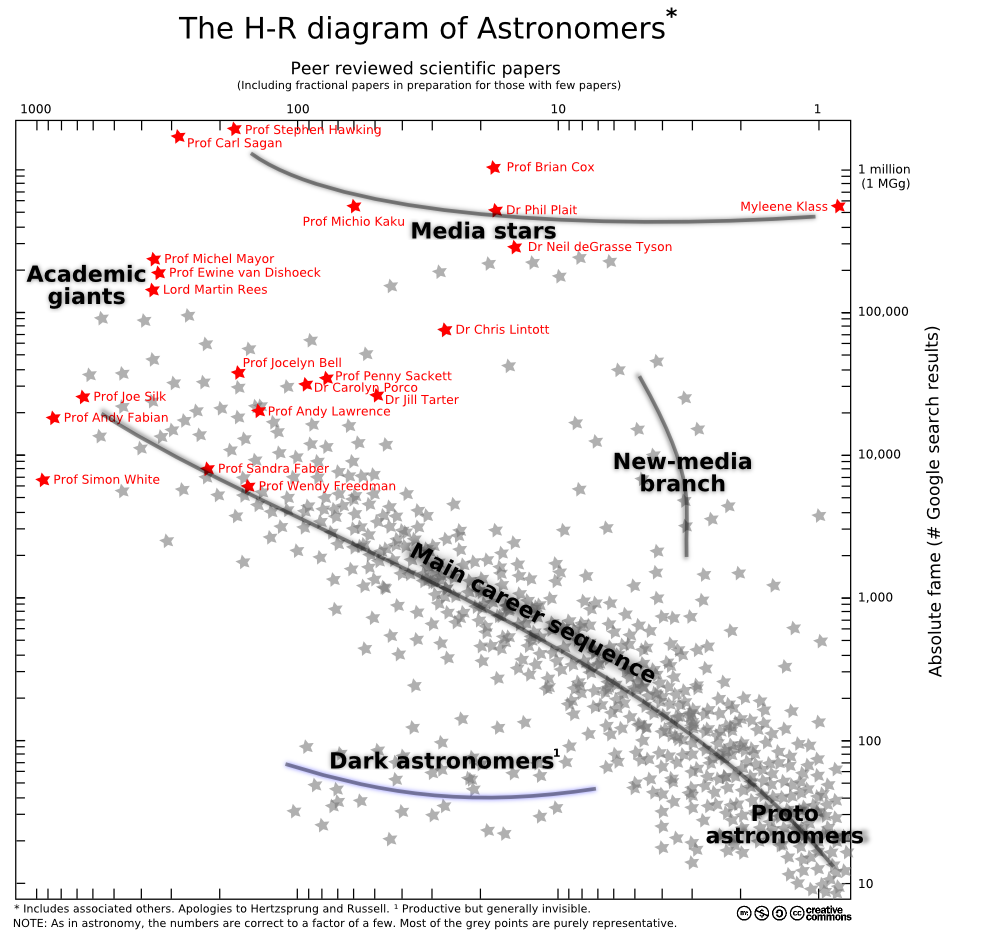
\includegraphics[width=0.8\linewidth]{figs/astronomos.png}
	\end{center}
\end{frame}

\subsection{Consulta de publicaciones}

\begin{frame}{Métricas de calidad}{Consulta de publicaciones}
	DBLP: \url{http://dblp.uni-trier.de/}\\
	Google My Citations: \url{http://scholar.google.com/}\\
	Publish or perish (exe): \url{http://www.harzing.com/pop.htm}
\end{frame}


\section{Proceso de publicación}
\subsection[Pasos]{Pasos de una publicación}
\begin{frame}{Proceso de publicación} {Pasos para publicar}
	\begin{enumerate}
		\item Decidir dónde publicar
		\item Buscar plantilla
		\item Escribir el artículo
		\item Enviar el artículo
		\item Revisión de pares
		\item Enviar CRC
		\item [Congreso] Presentación oral
	\end{enumerate}
\end{frame}

\subsection{Dónde publicar}

\begin{frame}{Proceso de publicación} {Dónde publicar: Seleccionar publicación}
	\begin{columns}
	\column{.5\textwidth}
	\begin{block}{Factores políticos}
	\begin{center}
	\begin{itemize}
		\item Velocidad de la revisión
		\item ¿Es un número especial?
		\item ¿El congreso tiene número especial?
		\item Conocidos
		\item Experiencia previa
		\item ¿Asiste gente interesante?
	\end{itemize}
	\end{center}
	\end{block}

	\column{.5\textwidth}
	\begin{block}{Factores científicos}
  	\begin{center}
	\begin{itemize}
		\item ``Topics''
		\item \alert{Impacto}
		\item Calidad
		\item Revisiones
		\item Realimentación
	\end{itemize}
	\end{center}
	\end{block}
	\end{columns}
\end{frame}

\begin{frame}{Proceso de publicación} {Dónde publicar: Editoriales y asociaciones científicas}
%	\begin{columns}
%	\column{.5\textwidth}
	\begin{block}{Editoriales}
	\begin{center}
  		\begin{center}
      	
\includegraphics[width=0.3\linewidth]{figs/springer.jpg}\hspace{1cm}
      	
\includegraphics[width=0.2\linewidth]{figs/elsevier.jpg}\hspace{1cm}
      	
\includegraphics[width=0.2\linewidth]{figs/wiley.jpg}
	    \end{center}
	\end{center}
	\end{block}

%	\column{.5\textwidth}
	\begin{block}{Asociaciones}
  		\begin{center}
      	
\includegraphics[width=0.3\linewidth]{figs/acm.png}\hspace{1cm}
      	
\includegraphics[width=0.3\linewidth]{figs/ieee.jpg}
	    \end{center}
	\end{block}
%	\end{columns}
\end{frame}

\subsection{Buscar plantilla}
\begin{frame}{Proceso de publicación} {Buscar plantilla}
	Todas las publicaciones ofrecen una \alert{plantilla} e \alert{instrucciones}
	\begin{itemize}
		\item \alert{\LaTeX es el formato estándar en ciencia}
		\item A veces se admite formato Word (es raro)
		\item Sí o sí, es necesario aprender \LaTeX (y esto es bueno)
	\end{itemize}
	\bigskip
	Cómo redactar un paper será tratado en una sesión específica
\end{frame}

\subsection{Envío de un artículo}
\begin{frame}{Proceso de publicación} {Envío de un artículo}
	En una palabra: \textit{On-line}
	\begin{itemize}
		\item Todas las editoriales tienen un plataforma integral
		\item Gestión de ciclo de vida en la plataforma
		\item Designar a un autor responsable (\textit{corresponding author})
		\item Enviar un paper a veces no trivial
			\begin{itemize}
			\item Puede ir de rellenar un formulario con el PDF ... a compilar el documento \textit{en el servidor}
			\item Un par de horas mínimo
			\item Rarezas: \textit{Cover letter}, sugerir editores, etc.
			\end{itemize}
		\item Se asigna un identificador a cada paper
	\end{itemize}
\end{frame}

\subsection{Revisión entre pares}

\begin{frame}{Proceso de publicación}{Revisión de pares: Motivos}
   \begin{block}{Motivos}
   	\begin{itemize}
		\item Asegurar la calidad
		\item Verificar la validez científica
		\item Asegurar la originalidad de las contribuciones
		\item Aportar realimentación a los autores $\Rightarrow$ \alert{Mejorar la calidad}
	\end{itemize}
   \end{block}
\end{frame}

\begin{frame}{Proceso de publicación}{Revisión de pares: Criterios (I)}
	Criterios científicos:
   	\begin{itemize}
		\item ¿El trabajo es relevante? 
		\item ¿El resultado es original?
		\item ¿La metodología es rigurosa?
		\item ¿Experimentación apropiada?
		\item ¿Las conclusiones están avaladas por la evidencia?
		\item ¿Está revisado el trabajo relacionado?
		\item ¿La presentación de resultados es adecuada?
		\item ¿El tema es del interés de la audiencia de la publicación?
	\end{itemize}
\end{frame}

\begin{frame}{Proceso de publicación}{Revisión de pares: Criterios (II)}
	Criterios formales:
   	\begin{itemize}
		\item ¿El artículo está bien escrito?
		\item ¿Todas las referencias están citadas?
		\item ¿Referencias duplicadas o mal escritas?
		\item ¿Referencias sin actualizar?
		\item ¿Todas las figuras son citadas?
	\end{itemize}
	\alert{Siempre se mira: ¡Mucho cuidado!}
\end{frame}

\begin{frame}{Proceso de publicación}{Revisión de pares: Criterios (III)}
	 \begin{center}
	    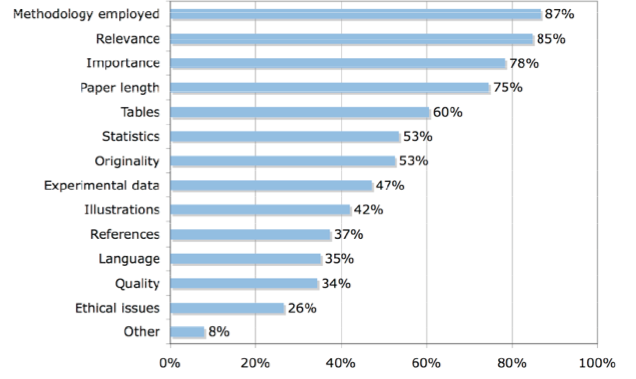
\includegraphics[width=0.9\linewidth]{figs/revision.png}
 	 \end{center}
\end{frame}

\begin{frame}{Proceso de publicación}{Revisión de pares: La decisión}
	El editor, con entre dos y cinco revisiones, toma una decisión y se notifica al autor
 	\begin{block}{Decisiones}
   		\begin{itemize}
			\item Aceptado
			\item Aceptado con cambios menores (\textit{minor revision})
			\item Aceptado con cambios mayores (\textit{major revision})
			\item Rechazado
		\end{itemize}
	\end{block}
	En congreso suele ser aceptado/rechazado

	\alert{Casi siempre hay que hacer una revisión}
\end{frame}

\begin{frame}{Proceso de publicación}{Revisión de pares: La revisión}
  	\begin{itemize}
		\item Todos las sugerencias deben ser introducidas
		\begin{itemize}
			\item Si no se hace, debe justificarse en una carta al editor
		\end{itemize}
		\item Los cambios deberían ser señalados (p.e. negrita)
		\item Una vez hecha la revisión, se reenvía junto a una carta
	\end{itemize}

	%\alert{Normalmente, siempre hay que hacer una revisión}
\end{frame}

\begin{frame}{Proceso de publicación}{Enviar CRC}
  	\begin{itemize}
		\item Aceptado el artículo, se envía una prueba en PDF al autor
			\begin{itemize}
			\item El autor debe comprobar errores de procesado
			\item No se admiten grandes cambios
			\end{itemize}
		\item CRC: \textit{Camera Ready Copy}
		\begin{itemize}
			\item Versión final que se incluye en la revista o actas
		\end{itemize}
		\item El editor envía el artículo final
		\begin{itemize}
			\item Incluye número de página
			\item Es citable
			\item Normalmente aparece \textit{on-line} antes que en papel
			\item Algunas revistas regalan varias copias en papel (\textit{hard copy}), otras las venden
		\end{itemize}
	\end{itemize}

	%\alert{Normalmente, siempre hay que hacer una revisión}
\end{frame}

\begin{frame}{Proceso de publicación}{Presentación oral}
  	\begin{itemize}
		\item Obviamente, es exclusivo a congresos
		\item Se agrupan ponencias de áreas temáticas similares
			\begin{itemize}
			\item Se las llama \alert{sesión} (\textit{session})
			\item 4 ó 5 ponencias en dos horas
			\item Estándar: 20 min. presentación + 10 min. preguntas
			\end{itemize}
		\item Cada sesión es dirigida por un \alert{chairman}
			\begin{itemize}
			\item Dirige la sesión
			\item Presenta a los ponentes
			\item Vigila que se cumplan los tiempos
			\item Normalmente, si nadie pregunta nada, hace una pregunta de cortesía
			\end{itemize}
	\end{itemize}

	%\alert{Normalmente, siempre hay que hacer una revisión}
\end{frame}



\end{document}
